\documentclass[border=2pt]{standalone}
\usepackage{tikz}
\usetikzlibrary{arrows.meta,positioning,shapes.symbols}
\begin{document}
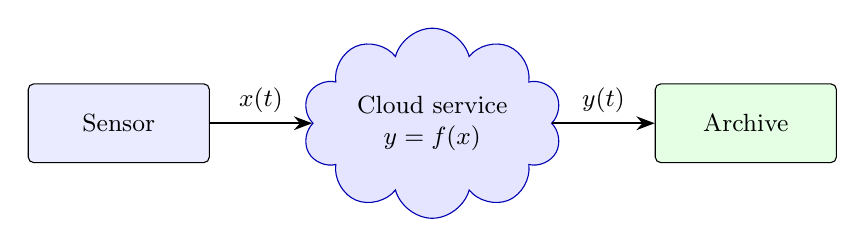
\begin{tikzpicture}[
  >=Stealth,
  node distance=13mm,
  every node/.style={font=\small},
  stage/.style={draw,rounded corners=2pt,minimum width=23mm,minimum height=10mm},
  link/.style={->,thick}
]
  \node[stage,fill=blue!8] (sensor) {Sensor};
  \node[cloud,cloud puffs=10,cloud puff arc=150,aspect=1.7,
        draw=blue!70!black,fill=blue!10,minimum width=32mm,minimum height=17mm,
        align=center,right=of sensor] (service) {Cloud service\\$y=f(x)$};
  \node[stage,fill=green!10,right=of service] (archive) {Archive};
  \draw[link] (sensor) -- node[above] {$x(t)$} (service);
  \draw[link] (service) -- node[above] {$y(t)$} (archive);
\end{tikzpicture}
\end{document}
